\documentclass{beamer}
%pdflatex -shell-escape my_document.tex

\usetheme{default}
\usecolortheme{rose}
\usefonttheme{serif}
%\usefonttheme{structureitalicsserif}

\definecolor{verdeuni}{rgb}{0.7,0.73437,0.55856}
\setbeamertemplate{headline}[verdeuni]
%\setbeamercovered{highly dinamic}
%\usepackage{eso-pic}

\usepackage{minted}

\usepackage{stmaryrd}
\usepackage{local-macros2}
\newcommand{\distance}[2]{|#1 - #2|}
\newcommand{\outputdistance}[2]{||#1 - #2||}
%\newcommand{\x}{\vect{x}} 		% Arbitrary input
%\newcommand{\xt}{\hat{\x}} 		% Training input
\newcommand{\xs}{\x} 			% Sampled input
\newcommand{\xp}{\tilde{\x}} 	% Perturbed input

%\newcommand{\y}{\vect{y}} 		% Arbitrary output
\newcommand{\yt}{\hat{\y}} 		% Training output
\newcommand{\ys}{\y} 			% Sampled output



\newcommand{\SR}[2]{SR(#1, #2)} % Standard robustness
\newcommand{\LR}[2]{LR(#1, #2)} % Lipschitz robustness
\newcommand{\CR}[1]{CR(#1)} % Classification robustness
\newcommand{\SCR}[2]{SCR(#1,#2)} % Approximate class. robustness

\usepackage{amsfonts,amsmath,amssymb,amsthm}
\usepackage[all]{xy}
\usepackage{array,url}
\usepackage{textcomp,textgreek}
\usepackage{pgfplots}
\usepackage{float}
\pgfplotsset{width=5cm,compat=1.9}
\usepackage{mdframed,wrapfig,subcaption}
%\usepackage[font=footnotesize,labelfont=it
%\usepackage[latin1]{inputenc}
\usepackage{babel}
\usepackage{color}
%\usepackage{url}
\usepackage{hyperref}
\usepackage{fancyvrb}
%\usepackage{tikz}
\usepackage{alltt}
%\usepackage{etex, xy}
%\usepackage{cibeamer}
\usepackage{tikz}
\usetikzlibrary{arrows,shapes}
%\xyoption{all}
%\usepackage{listings}
%\input macro
\usepackage{cancel, comment}
\usepackage{verbatim}
\usepackage{slashbox}
\usepackage{ulem}

\newcommand{\tikzmark}[1]{\tikz[remember picture] \node[coordinate] (#1) {#1};}
\newcommand{\semitransp}[2][35]{\color{fg!#1}#2}

\usepackage[absolute,overlay]{textpos}
\beamertemplatenavigationsymbolsempty
\usepackage{ijcnn-diagram}

\usepackage[all]{foreign}

\newcommand{\fstar}{F$^\ast$\xspace}
\newcommand{\starchild}{StarChild\xspace}
\newcommand{\lazuli}{Lazuli\xspace}
\newcommand{\sapphire}{Sapphire\xspace}
\newcommand{\cL}{{\cal L}}
%\newcommand{\Real}{{\mathbb R}}
\usepackage{makecell}
\DeclareMathOperator{\linear}{linear}
\DeclareMathOperator{\relu}{relu}
\DeclareMathOperator{\sigmoid}{sigmoid}
\DeclareMathOperator{\softmax}{softmax}
\DeclareMathOperator{\neuron}{neuron}
\DeclareMathOperator{\truthy}{truthy}
\DeclareMathOperator{\falsey}{falsey}
\DeclareMathOperator{\neurontest}{test}
\usepackage{ellipsis}
\renewcommand{\ellipsisgap}{-0.25em}

\usepackage{soul}
\makeatletter
\let\HL\hl
\renewcommand\hl{%
  \let\set@color\beamerorig@set@color
  \let\reset@color\beamerorig@reset@color
  \HL}
\makeatother

%\usetikzlibrary{decorations.pathreplacing,shapes.arrows}
\newcommand\BackgroundPicture[1]{%
  \setbeamertemplate{background}{%
   \parbox[c][\paperheight]{\paperwidth}{%
      \vfill \hfill
\includegraphics[width=1\paperwidth,height=1\paperheight]{#1}
        \hfill \vfill
     }}}
\usepackage{xcolor,colortbl}
%\usepackage{listings}
\definecolor{Gray}{gray}{0.85}

%\setbeamertemplate{footline}[frame number]

%\newcommand{\rrdc}{\mbox{\,\(\Rightarrow\hspace{-9pt}\Rightarrow\)\,}} % Right reduction
%\newcommand{\lrdc}{\mbox{\,\(\Leftarrow\hspace{-9pt}\Leftarrow\)\,}}% Left reduction
%\newcommand{\lrrdc}{\mbox{\,\(\Leftarrow\hspace{-9pt}\Leftarrow\hspace{-5pt}\Rightarrow\hspace{-9pt}\Rightarrow\)\,}} % Equivalence
%\DeclareMathOperator{\id}{Id}
%\newcommand{\Zset}{\mathbb{Z}}
%\newcommand{\Bset}{\mathbb{Z}_2}

\setbeamertemplate{navigation symbols}{}

\mode<presentation>
\title[Vehicle Tutorial Chapter 4]{Vehicle Tutorial Chapter 4: Property-Driven Training}
%\subtitle{in Neuro-Symbolic Landscape}
\author[Vehicle]{Today's presentors: Ekaterina Komendantskaya and Luca Arnaboldi  (live), Matthew Daggitt (online), on behalf of the Vehicle team}
\institute[]{}

\date[]{}

%\logo{
\includegraphics[width=6cm]{LaivLogolong.png}}

\AtBeginSection[]
{
  \begin{frame}
    \frametitle{Table of Contents}
    \tableofcontents[currentsection]
  \end{frame}
}

\begin{document}
\BackgroundPicture{logo1.png}

\begin{frame}
\titlepage
\end{frame}

\begin{frame}
\frametitle{In this chapter...}

We will discuss:

\begin{itemize}[<+->]
\item  ...  why training is part of verification of neural networks
\item ... what choices exist for achieving this, generally
\item ... what choice \textbf{Vehicle} makes in this respect
\item ... theoretical and practical issues with the chosen methods, and \textbf{Vehicle}'s
take on them
\end{itemize}

\end{frame}


\begin{frame}
\frametitle{Recap: four PL problems}

\pause
\begin{itemize}
\item[$I^O$] \alert{Interoperability -- properties are not portable between training/counter-example search/ verification.}

\item[$I^{P}$] Interpretability -- code is not easy to understand.

\item[$I^{\int}$] Integration -- properties of networks cannot be linked to larger control system properties.

\item[$E^G$] Embedding gap -- little support for translation between problem space (as in original spec) and input space (at neural network level).
\end{itemize}
\end{frame}


    \begin{frame}[fragile]
\frametitle{Why Training is a part of Verification?}

\begin{minted}[fontsize=\footnotesize]{vehicle}
vehicle verify \
  --specification acasXu.vcl \
  --verifier Marabou \
  --network acasXu:acasXu_1_7.onnx \
  --property property3

Verifying properties:
property3 [==========================================] 1/1 queries
  result:  counterexample found
  x: [1799.9886669999978, 1.9509286320000003e-2, 
                        3.09999732192, 980.0, 1017.6036]
\end{minted}

\end{frame}

   \begin{frame}
\frametitle{Why Training is a part of Verification?}

For Chapter 3 exercise on verifying a small Fashion MNIST network, the answer would be:

\footnotesize{
\begin{tabular}{|p{0.2\textwidth}|p{0.15\textwidth}|p{0.15\textwidth}|p{0.15\textwidth}| p{0.15\textwidth}|}
		\hline
& 	$\epsilon = 0.01$ & $\epsilon = 0.05$ & $\epsilon = 0.1$ & $\epsilon = 0.5$ \\ \hline \hline

Success rate: & 82.6 \% (413/500) &	29.8 \% (149/500) &	3.8 \% (19/500) & 	0 \% (0/500)\\		
		 \hline
	\end{tabular}}


\end{frame}

\begin{frame}
  \frametitle{A few words on the context}

  \begin{itemize}
  \item[1943] Perceptron by McCullogh and Pitts
  \item[90-2000] Rise of machine learning applications
  \item[2013]
   {\scriptsize
 \begin{thebibliography}{99}
 \beamertemplatearticlebibitems
  \bibitem{2}{C.~Szegedy, W.~Zaremba, I.~Sutskever, J.~Bruna, D.~Erhan,
I.~Goodfellow, and R.~Fergus.  Intriguing properties of neural networks. 2013. (10000+ citations on GS)}
\end{thebibliography}}

\item[2013-..] Tens of thousands of papers on adversarial training

  (in the attack-defence style)
    {\scriptsize
 \begin{thebibliography}{99}
   \beamertemplatearticlebibitems
   \bibitem{3}{A.~C.~Serban, E.~Poll, J.~Visser.
Adversarial Examples - A Complete Characterisation of the Phenomenon. 2019.}
\end{thebibliography}}

\pause

\item[2017] First Neural network verification attempts
    {\scriptsize
 \begin{thebibliography}{99}
   \beamertemplatearticlebibitems
    \bibitem{4}{G.~Katz, C.W.~Barrett, D.L.~Dill, K.~Julian, M.J.~Kochenderfer:
      Reluplex: An Efficient SMT Solver for Verifying Deep Neural Networks. CAV (1) 2017: 97-117.}
    \bibitem{5}{ X. Huang, M. Kwiatkowska, S. Wang, M. Wu. Safety Verification of Deep Neural Networks. CAV (1) 2017: 3-29.}
\end{thebibliography}}


\item[2017-..] Hundreds of papers on neural network verification

  \end{itemize}
\end{frame}




\begin{frame}
  \frametitle{}



  \begin{block}{ Training for Robustness}
   % \begin{center}

    %  \end{center}
    \end{block}

    \pause
    Training generally:

    \begin{enumerate}
    \item depends on data
    \item depends on loss functions
      \item some other parameters like shape of the functions
      \end{enumerate}
    
\end{frame}





\begin{frame}[fragile]
  \frametitle{1. Data Augmentation}
  Suppose we are given a data set $\mathcal{D} =  \{(\x_1, \y_1), \ldots , (\x_n, \y_n)\}$.
  Prior to training, generate new training data samples close to existing data and label them with the same output as the original data.
      {\scriptsize
 \begin{thebibliography}{99}
   \beamertemplatearticlebibitems
    \bibitem{6}{C. Shorten, T.M. Khoshgoftaar: 
       A survey on image data augmentation for deep learning. J.
Big Data 6, 60 (2019)}
\end{thebibliography}}

\pause

\begin{center}

  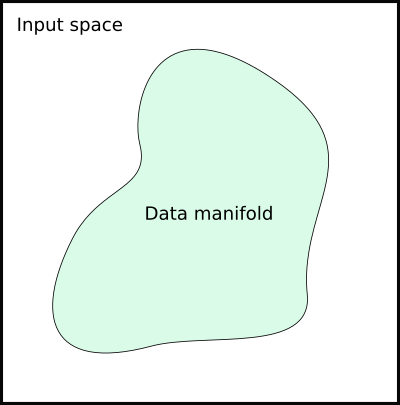
\includegraphics[width=5cm]{Images/SR-vs-CR-1.png}

  \end{center}
  
\end{frame}


\begin{frame}[fragile]
  \frametitle{1. Data Augmentation}
  Suppose we are given a data set $\mathcal{D} =  \{(\x_1, \y_1), \ldots , (\x_n, \y_n)\}$.
  Prior to training, generate new training data samples close to existing data and label them with the same output as the original data.
      {\scriptsize
 \begin{thebibliography}{99}
   \beamertemplatearticlebibitems
    \bibitem{6}{C. Shorten, T.M. Khoshgoftaar: 
       A survey on image data augmentation for deep learning. J.
Big Data 6, 60 (2019)}
\end{thebibliography}}


\begin{center}

  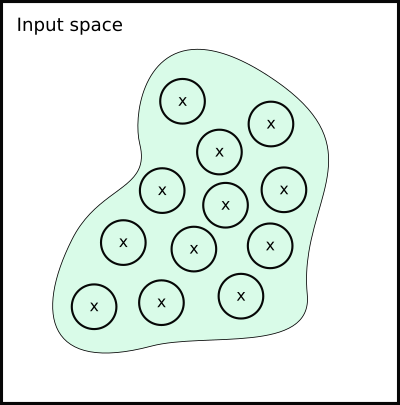
\includegraphics[width=5cm]{Images/SR-vs-CR-2.png}

  \end{center}
  
\end{frame}




\begin{frame}[fragile]
  \frametitle{However,}


\begin{center}

  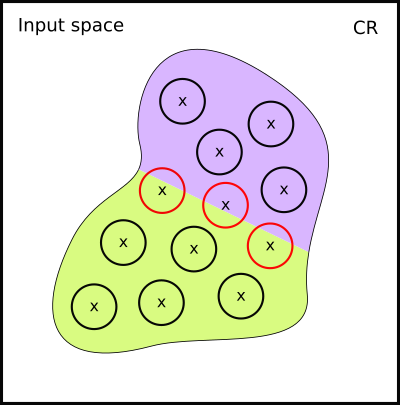
\includegraphics[width=5cm]{Images/SR-vs-CR-4.png}

  \end{center}
  
\end{frame}


\begin{frame}[fragile]
  \frametitle{However,}



\begin{center}

  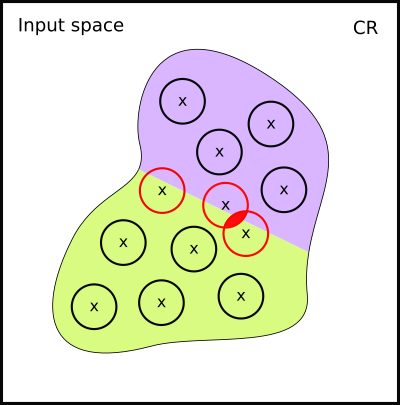
\includegraphics[width=5cm]{Images/SR-vs-CR-5.png}

  \end{center}
  
 \end{frame}

 \begin{frame}[fragile]
  \frametitle{Adversarial Training}



\begin{center}

  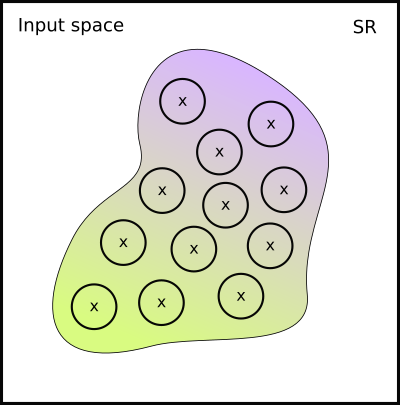
\includegraphics[width=5cm]{Images/SR-vs-CR-3.png}

  \end{center}
  
 \end{frame}


\begin{frame}
  \frametitle{2. Solutions Involving Loss Functions}
Given a data set $\mathcal{D} $,  a function  ${f: \Real^n \rightarrow \Real^m}$,
	a loss function $\losssymbol: \Real^n \times \Real^m \rightarrow \Real$ computes a penalty proportional to the difference between the output of $f$ on a training input $x$ and a desired output $y$.\pause


\begin{example}[Cross Entropy Loss Function]
	\label{eq:cross-entropy}
	Given a function  ${f: \Real^n \rightarrow [0,1]^m}$, the cross-entropy loss is defined as 
	\begin{equation}\label{eq:ce}
	\losssymbol_{ce}(\x, \y) = - \sum_{i=1}^{m} \y_i \; \log(f(\x)_i)
	\end{equation}
	where $\y_i$ is the true probability for class $i$ and $f(\x)_i$ the probability for class $i$ as predicted by $f$ when applied to $\x$.
\end{example}

\end{frame}

 

\begin{frame}
  \frametitle{2. Adversarial Training  for Robustness}

  \begin{itemize}
  \item  \emph{gradient descent}  minimises loss $\lossfn(\xt, \y)$ between the predicted value $f_{\theta}(\xt)$ and the true value $\y$, for each entry $(\xt, \y)$ in $\mathcal{D}$:  
  $$ \min_{\theta} \lossfn(\xt, \y) $$
  \pause
  \item instead minimise the loss with respect to the worst-case perturbation of each sample in $\mathcal{D}$.
\begin{itemize}
     \item Replace the standard training objective with:
%\begin{equation}
$$\min_{\theta} \max_{\forall \xs : \distance{\xs}{\xt} \leq \epsilon} \lossfn(\xs, \y)$$
 \item often referred to as the method of \emph{``projected gradient descent"} (PGD)

\end{itemize}
\end{itemize}

 {\scriptsize
   \begin{thebibliography}{99}
        \beamertemplatearticlebibitems
    \bibitem{7}
I.J. Goodfellow, J. Shlens, C. Szegedy: Explaining and harnessing adversarial examples. 3rd International Conference on Learning Representations,
ICLR 2015, San Diego, CA, USA, May 7-9, 2015, Conference Track Proceedings (2015)
 \end{thebibliography}}

\end{frame}


    \begin{frame}
      \frametitle{3. Lipshitz Continuity}

      Optimise for: 
      
  \begin{equation*}
    \label{eq:lipschitz-robustness}
    \forall \xs: \distance{\xs}{\xt} \leq \epsilon \Rightarrow \distance{f(\xs)}{f(\xt)} \leq L \distance{\xs}{\xt}
  \end{equation*}

   {\scriptsize
   \begin{thebibliography}{99}
        \beamertemplatearticlebibitems
    \bibitem{7}
P. Pauli, A. Koch, J. Berberich, P. Kohler, F. Allgower: Training robust neural networks
using Lipschitz bounds. IEEE Control Systems Letters (2021)
\bibitem{8} H. Gouk, E. Frank, B. Pfahringer, M.J. Cree: Regularisation of neural networks by enforcing Lipschitz continuity. Machine Learning 110(2), 393–416 (2021)
\end{thebibliography}}


and much more...

    \end{frame}


\begin{frame}
\frametitle{}

\begin{alertblock}{Ok, great!}
 Machine Learning Community knows how to make our networks robust, and maybe even verifiable!
\end{alertblock}
\pause
But remember: 

\begin{block}{}
\begin{itemize}
\item[$I^O$] \alert{Interoperability -- properties are not portable between training/counter-example search/ verification.}

\item[$I^{P}$] \alert{Interpretability} $\ldots$

\item[$I^{\int}$] Integration $\ldots$

\item[$E^G$] Embedding gap $\ldots$
\end{itemize}
\end{block}
\end{frame}

\begin{frame}
  \frametitle{Interpretation of adversarial training in connection to verification properties}

  
    \begin{itemize}[<+-|alert@+>]
      \item Recall the epsilon ball robustness:
      
       $\forall \x \in \mathbb{B}(\hat{\x}, \epsilon). \ \alert{robust}(f(\x)) $

        \item We can map different kinds of adversarial training to formal properties:
          	\begin{tabular}{p{3.5cm}|p{5.5cm}} 
		%\toprule
		Training style & Definition of \textbf{$robust$}  \\ \hline \hline
		%\midrule
		Data Augmentation & 	$ argmax\ f(\x) = c$  \\ \hline
		Adversarial Training & 	$ |f(\x) - f(\hat{\x})| \leq \delta$ \\ \hline
          Lipschitz Continuity & 	$ |f(\x) - f(\hat{\x})| \leq L|\x-\hat{\x}|$  \\ \hline
          ... & ... \\
		%Approximate CR (ACR) & 	$\forall X: ||X-\hat{X}|| \leq \epsilon \Longrightarrow f(X)_c \geq \eta$  \\
		%\bottomrule
	\end{tabular}
        \end{itemize}
        
        
       {\scriptsize
 \begin{thebibliography}{99}
   \beamertemplatearticlebibitems
    \bibitem{6}{M. Casadio, E. Komendantskaya, M. L. Daggitt, W. Kokke,
G. Katz, G.~Amir, and I.~Rafaeli. 2022. Neural Network Robustness as a Verification Property:
A Principled Case Study. CAV'22.}
\end{thebibliography}}
 
    
  \end{frame}




\begin{frame}[fragile]
\frametitle{Problem Recap}

\begin{itemize}
\item one kind of robustness does not necessarily imply another;

\item It is easy to get it wrong, and,  while optimising for a \alert{wrong kind} of robustness, achieve little in verification success rates

\item And what to do with properties that are not $\epsilon$-ball robustness? 
\end{itemize}
\pause

\begin{block}{}
\begin{itemize}
\item[$I^O$] \alert{Interoperability -- properties are not portable between training/counter-example search/ verification.}

\item[$I^{P}$] \alert{Interpretability} $\ldots$

\item[$I^{\int}$] Integration $\ldots$

\item[$E^G$] Embedding gap $\ldots$
\end{itemize}
\end{block}
\end{frame}

\begin{frame}
	\frametitle{The solution we are looking for}
	
	
	\begin{figure}[t]
		\begin{center}
			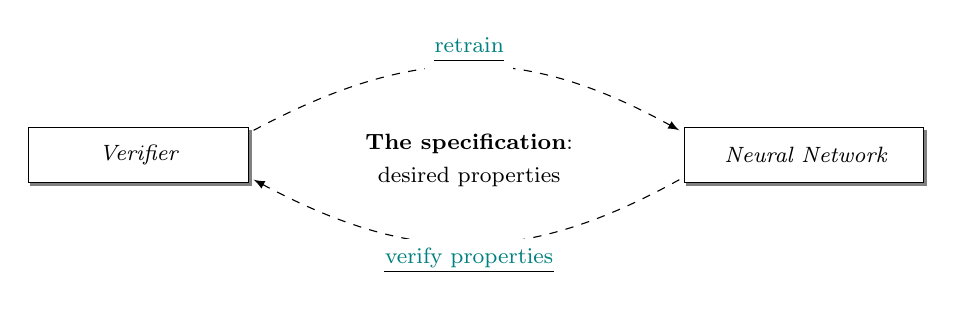
\begin{tikzpicture}[scale=.7]
				
				\draw[fill=gray,draw=gray] (-2.95,.45) rectangle (1.05,-.55);  
				\draw[fill=white] (-3,.5) rectangle (1,-.5); 
				\node (0,0) { };
				\draw (-1,0) node {{\footnotesize \it Verifier} };
				
				\draw[fill=gray,draw=gray] (8.95,.45) rectangle (13.30,-.55);  
				\draw[fill=white] (8.9,.5) rectangle (13.25,-.5); 
				\draw (11.1,0) node{{\footnotesize \it Neural Network}};
				
				
				\draw (5,0.2) node{\footnotesize{\textbf{The specification}:}};
				\draw (5,-0.4) node{\footnotesize{desired properties}};
				
				
				\draw[latex-,shorten <=2pt,shorten >=2pt,dashed] (8.9,.4) .. controls (6,2) and (4,2) .. (1,.4); 
				\draw (5,2.3) node[anchor=north,fill=white]{\emph{\footnotesize{\textcolor{teal}{retrain}}}};
				
				\draw[latex-,shorten <=2pt,shorten >=2pt,dashed] (1,-.4) .. controls (4,-2) and (6,-2) .. (8.9,-.4); 
				\draw (5,-2.3) node[anchor=south,fill=white]{\emph{\footnotesize{\textcolor{teal}{verify properties}}}}; 
			\end{tikzpicture}
		\end{center}
	\end{figure}
\end{frame}

\begin{frame}
\frametitle{In Vehicle terms,}


\begin{center}
\begin{tikzpicture}[thick,
    set/.style = {circle,
        minimum size = 3cm}]

% Set A
\node[rectangle,draw] (A) at (1.5,5) {\alert{Property in Vehicle}};

\node[rectangle,draw] (B) at (-3,2) {\alert{Training}};
\node[text width=1cm, align=center] at (-3,0) {\alert{DL2 or other DL (native)}};

\node[rectangle,draw, dashed,text width=1.4cm] (C) at (0,2) {\alert{Counter-example search}};
\node[text width=1cm, align=center] at (0,0) {\alert{PGD FGSM etc.}};

\node[rectangle,draw] (D) at (3,2) {Verification};
\node[text width=1.4cm, align=center] at (3,0) {Marabou Eran etc.};

\node[rectangle,draw] (E) at (6,2) {Integration};
\node[text width=2cm, align=center] at (6,-0.3) {Agda Imandra KeymaeraX etc.};

\draw [->] (A) edge (B);
\draw [->, dashed] (A) edge (C);
\draw [->] (A) edge (D);
\draw [->] (A) edge (E);
%\draw [->, dashed] (A) edge (C);
\draw [->] (B) edge (C);
\draw [->] (C) edge (D);
\draw [->] (D) edge (E);

\onslide<1->{
\node[rectangle,draw,fill=normal text.bg] (D) at (1.5,4) {Analysis \& informative error messages};
}


\end{tikzpicture}
\end{center}
\end{frame}

\end{document}

\begin{frame}[fragile]
\frametitle{Values}

Types for values are automatically inferred by \textbf{Vehicle}. For example, we can declare the number $\pi$ and its type will be inferred as rational:

\begin{minted}[fontsize=\small]{vehicle}

pi = 3.141592
\end{minted}
\end{frame}

\begin{frame}[fragile]
\frametitle{Working with vectors}
\begin{itemize}
\item some input or output pre-processing maybe expected when defining a neural network.

\begin{example}
It is assumed that the ACAS Xu inputs and outputs are normalised, i.e. the network does not work directly with units like $m/s$. However, the specifications  we want to write should ideally concern the original units.
\end{example}

\pause


\item This is an instance of \emph{``problem space / input space mismatch"}

\item ... that is very common in neural net verification

\item
Being able to reason about problem space (alongside the input space) is a feature that distinguishes \textbf{Vehicle} from
majority of the mainstream neural network verifiers
\end{itemize}
\end{frame}

\begin{frame}[fragile]
\frametitle{Vector normalisation}
For clarity, we define a new type synonym for unnormalised input vectors which are in the problem space.
\begin{minted}[fontsize=\footnotesize]{vehicle}

type UnnormalisedInputVector = Vector Rat 5

\end{minted}

Next we define the range of the inputs that the network is designed
to work over.

\begin{minted}[fontsize=\footnotesize]{vehicle}

minimumInputValues : UnnormalisedInputVector
minimumInputValues = [0.0, -pi , -pi , 100.0, 0.0]

maximumInputValues : UnnormalisedInputVector
maximumInputValues = [60261.0, pi, pi, 1200.0, 1200.0]

meanScalingValues : UnnormalisedInputVector
meanScalingValues = [19791.091, 0.0, 0.0, 650.0, 600.0]
\end{minted}
\end{frame}



\begin{frame}[fragile]
\frametitle{Vector manipulation}
An alternative method to vector definition is to use the `foreach` constructor, which is used to provide a value for each `index i`.
\begin{minted}[fontsize=\footnotesize]{vehicle}

minimumInputValues : UnnormalisedInputVector
minimumInputValues = foreach i . 0

\end{minted}
Let us see how  `foreach` works with vector indexing.

We can now define the normalisation function that takes an input vector and
returns the unnormalised version.

\begin{minted}[fontsize=\footnotesize]{vehicle}

normalise : UnnormalisedInputVector -> InputVector
normalise x = foreach i .
  (x ! i - meanScalingValues ! i) / (maximumInputValues ! i)
\end{minted}

\pause
... our first acquaintance with functions!

\end{frame}



\begin{frame}[fragile]
\frametitle{Functions and types}
\begin{minted}[fontsize=\footnotesize]{vehicle}
<name> : <type>
<name> [<args>] = <expr>

\end{minted}
Functions make up the backbone of the \textbf{Vehicle} language.
\pause
\begin{minted}[fontsize=\footnotesize]{vehicle}

validInput : UnnormalisedInputVector -> Bool
validInput x = forall i .
  minimumInputValues ! i <= x ! i <= maximumInputValues ! i

\end{minted}

\pause

\begin{block}{Our first acquaintance with predicates and quantifiers!}
 One of the main advantages of \textbf{Vehicle} is that it can be used to state and prove specifications that describe the network’s behaviour over an infinite set of values.
\end{block}

\end{frame}



\begin{frame}[fragile]
\frametitle{Functions and types}

\begin{block}{Function Composition: Exercise}

What are the types of functions `acasXu`  and `normalise`:

\begin{minted}[fontsize=\footnotesize]{vehicle}
normAcasXu : UnnormalisedInputVector -> OutputVector
normAcasXu x = acasXu (normalise x)
\end{minted}
\end{block}

\end{frame}

\begin{frame}[fragile]
\frametitle{Pre-defined functions and predicates}
We have already used:
\begin{minted}[fontsize=\footnotesize]{vehicle}
*
/
!
<=
\end{minted}

\begin{block}{Exercise}
\footnotesize{What do they stand for?}
\end{block}
\end{frame}



\begin{frame}[fragile]
\frametitle{Lets verify ACAS Xu!}
\begin{minted}[fontsize=\footnotesize]{vehicle}
distanceToIntruder = 0   -- measured in metres
angleToIntruder    = 1   -- measured in radians
intruderHeading    = 2   -- measured in radians
speed              = 3   -- measured in metres/second
intruderSpeed      = 4   -- measured in meters/second

clearOfConflict = 0
weakLeft        = 1
weakRight       = 2
strongLeft      = 3
strongRight     = 4
\end{minted}
\footnotesize{
The fact that all vector types come annotated with their size means that it
 is impossible to mess up indexing into vectors, e.g. if you changed
 `distanceToIntruder = 0` to `distanceToIntruder = 5` the specification would
 fail to type-check.}



\end{frame}

\begin{frame}[fragile]
\frametitle{Property 3}


\footnotesize{\textbf{If the intruder is \emph{directly ahead} and is moving towards the
 ownship, the score for COC will not be minimal.}}

\pause

\begin{minted}[fontsize=\footnotesize]{vehicle}
directlyAhead : UnnormalisedInputVector -> Bool
directlyAhead x =
  1500  <= x ! distanceToIntruder <= 1800 and
  -0.06 <= x ! angleToIntruder    <= 0.06
\end{minted}
\pause
\begin{block}{Exercise!}
\footnotesize{
\begin{enumerate}
\item
Can you identify whether the specification is written in terms of input space or problem space? How do you know?
\item Can you spot another pre-defined \textbf{Vehicle} function? What is it?
\end{enumerate}}
\end{block}

\end{frame}




\begin{frame}[fragile]
\frametitle{Property 3}

\footnotesize{\textbf{If the intruder is directly ahead and is \emph{moving towards} the
 ownship, the score for COC will not be minimal.}}

\pause

\begin{minted}[fontsize=\footnotesize]{vehicle}
movingTowards : UnnormalisedInputVector -> Bool
movingTowards x =
  x ! intruderHeading >= 3.10  and
  x ! speed           >= 980   and
  x ! intruderSpeed   >= 960
\end{minted}
\pause
\begin{block}{Exercise!}
\footnotesize{
\begin{enumerate}
\item Can you spot one more pre-defined \textbf{Vehicle} function? What is it?
\end{enumerate}}
\end{block}

\end{frame}

\begin{frame}[fragile]
\frametitle{There is little left to do!}

\footnotesize{
\textbf{If the intruder is directly ahead and is moving towards the
 ownship, the \emph{score for COC will not be minimal}.}}

\pause

\begin{minted}[fontsize=\footnotesize]{vehicle}
minimalScore : Index 5 -> UnnormalisedInputVector -> Bool
minimalScore i x = 
   forall j . i != j => normAcasXu x ! i < normAcasXu x ! j
\end{minted}
\pause
\begin{block}{Exercise!}
\footnotesize{
\begin{enumerate}
\item What kind of domain  `forall` ranges over? Is it finite or infinite?
\end{enumerate}}
\end{block}

\end{frame}


\begin{frame}[fragile]
\frametitle{There is little left to do!}

\footnotesize{
\textbf{If the intruder is directly ahead and is moving towards the
 ownship, the score for COC will not be minimal.}}

\pause

\begin{minted}[fontsize=\footnotesize]{vehicle}
@property
property3 : Bool
property3 = forall x . validInput x and 
                       directlyAhead x and 
                       movingTowards x =>
                       not (minimalScore clearOfConflict x)
\end{minted}
\pause
\begin{block}{Exercise!}
\footnotesize{
\begin{enumerate}
\item Can you guess the purpose of the syntax
\begin{minted}{vehicle}
@property
\end{minted}
?
\item What kind of domain  `forall` ranges over? Is it finite or infinite?
\end{enumerate}}
\end{block}

\end{frame}



\begin{frame}[fragile]
\frametitle{How to run Vehicle}
\begin{block}{Checklist}
\begin{enumerate}
\item a verifier installed (Marabou);
\item the actual network is supplied in an ONNX format
\item \textbf{Vehicle} is installed.
\end{enumerate}
\end{block}

\pause
\begin{minted}[fontsize=\footnotesize]{vehicle}
vehicle verify \
  --specification acasXu.vcl \
  --verifier Marabou \
  --network acasXu:acasXu_1_7.onnx \
  --property property3

Verifying properties:
property3 [==========================================] 1/1 queries
  result:  counterexample found
  x: [1799.9886669999978, 1.9509286320000003e-2, 
                        3.09999732192, 980.0, 1017.6036]
\end{minted}
\end{frame}





\begin{frame}
\frametitle{Vehicle ...}

 \textbf{ the part that we have seen}

\begin{center}
\begin{tikzpicture}[thick,
    set/.style = {circle,
        minimum size = 3cm}]

% Set A
\node[rectangle,draw] (A) at (1.5,5) {\alert{\textbf{Property in Vehicle}}};

\node[rectangle,draw] (B) at (-3,2) {Training};
\node[text width=1cm, align=center] at (-3,0) {DL2 ACT etc.};

\node[rectangle,draw, dashed, text width=1.4cm] (C) at (0,2) {Counter-example search};
\node[text width=1cm, align=center] at (0,0) {PGD FGSM etc.};

\node[rectangle,draw] (D) at (3,2) {\alert{\textbf{Verification}}};
\node[text width=1.4cm, align=center] at (3,0) {\alert{\textbf{Marabou}} Eran etc.};

\node[rectangle,draw] (E) at (6,2) {Integration};
\node[text width=2cm, align=center] at (6,-0.3) {Agda Imandra KeymaeraX etc.};

\draw [->] (A) edge (B);
\draw [->, dashed] (A) edge (C);
\draw [->] (A) edge (D);
\draw [->] (A) edge (E);

\draw [->] (B) edge (C);
\draw [->] (C) edge (D);
\draw [->] (D) edge (E);

\onslide<1->{
\node[rectangle,draw,fill=normal text.bg] (D) at (1.5,4) {\alert{\textbf{Analysis \& informative error messages}}};
}

\end{tikzpicture}
\end{center}
\end{frame}



\begin{frame}
\frametitle{Concluding Exercise}

Which of the four PL problems we addressed?

\begin{itemize}
\item[$I^O$] Interoperability -- properties are not portable between training/counter-example search/ verification.

\item[$I^{P}$] Interpretability -- code is not easy to understand.

\item[$I^{\int}$] Integration -- properties of networks cannot be linked to larger control system properties.

\item[$E^G$] Embedding gap -- little support for translation between problem space (as in original spec) and input space (at neural network level).
\end{itemize}
\end{frame}



\begin{frame}
\frametitle{Harder Exercise: ACAS Xu Property 1}

\small{
ACAS Xu Property 1 gives an idea how the {\it embedding gap}\\
 can arise not only when we reason about inputs, but also \\ the outputs of networks!
%In the previous lecture, we introduced ACAS Xu property 1.

\begin{itemize}
\item Can you formalise Property 1 in Vehicle?
\item Can you spot the instance of the embedding gap, this time concerning the network's output?
\end{itemize}}

\pause

\begin{definition}[ACAS Xu: Property 1]
\small{\it If the intruder is distant and is significantly slower than the ownship, the score of a COC advisory will always be below a certain fixed threshold:}



\begin{equation*}
\begin{array}{l}
(\rho \geq 55947.691) \wedge
(v_{own} \geq 1145) \wedge (v_{int} \leq 60)  \\
\Rightarrow \text{the score for COC is at most} 1500
\end{array}
\end{equation*}
\end{definition}

\pause

\begin{block}{Note:}
The ACAS Xu neural network outputs are scaled as follows: given an element $x$ of the output vector, we scale it as: $\frac{x - 7.518884}{373.94992}$. 
\end{block}

\end{frame}

\begin{frame}[fragile]
\frametitle{Next Lecture: $\epsilon$-ball Robustness}
 \begin{minted}[fontsize=\tiny]{vehicle}
type Image = Tensor Rat [28, 28]
type Label = Index 10
validImage : Image -> Bool
validImage x = forall i j . 0 <= x ! i ! j <= 1

@network
classifier : Image -> Vector Rat 10

advises : Image -> Label -> Bool
advises x i = forall j . j != i => classifier x ! i > classifier x ! j

@parameter
epsilon : Rat

boundedByEpsilon : Image -> Bool
boundedByEpsilon x = forall i j . -epsilon <= x ! i ! j <= epsilon

robustAround : Image -> Label -> Bool
robustAround image label = forall pertubation .
  let perturbedImage = image - pertubation in
  boundedByEpsilon pertubation and validImage perturbedImage =>
    advises perturbedImage label

@dataset
trainingImages : Vector Image n

@dataset
trainingLabels : Vector Label n

@property
robust : Vector Bool n
robust = foreach i . robustAround (trainingImages ! i) (trainingLabels ! i)
\end{minted}
\end{frame}

\end{document}


\begin{frame}
\frametitle{Plan for the rest of this tutorial}

\begin{itemize}
\item Before coffee break:
\begin{itemize}
%\item Brief introduction to \textbf{Vehicle} specification language 
\item \alert{Exercise session:} write and verify your own specs (with possibility to extend over the break)

\begin{itemize}
\item for writing a spec, install vehicle: just run 

\texttt{pip install vehicle-lang}

\item for verifying a spec, you also need Marabou installed 

\texttt{pip install maraboupy}

%(see Marabou pages)
\end{itemize}
\end{itemize}
\end{itemize}
\end{frame}


\begin{frame}
\frametitle{Exercises}

\begin{block}{Robustness (for those familiar with the problem)}
\footnotesize{
\begin{itemize}
\item Fill in missing code in the Robustness spec available at 
\url{https://github.com/vehicle-lang/tutorial}:\\
\url{exercises/Chapter 2. Getting Started/mnist-robustness}

\item Using the given neworks and data, verify robustness via Vehicle.
\end{itemize}}
\end{block}

\begin{alertblock}{Robustness (for those NOT familiar with the problem)}
\footnotesize{Study the chapter ``Proving Neural Network Robustness" here: \url{https://vehicle-lang.github.io/tutorial/}}
\end{alertblock}

\begin{block}{More ACAS Xu properties in the same spec}
\footnotesize{
\begin{itemize}
\item Extend the given ACAS Xu  specification with Property 1. 
The spec and network can be found at:  
\url{https://github.com/vehicle-lang/tutorial}, at \\
\url{examples/Chapter 2. Getting Started/acasXu}
\item Using the given neworks and data, verify the properties via Vehicle.
\end{itemize}}
\end{block}

\end{frame}



\end{document}
